%!TEX root = ../vkr.tex

\section{Обзор дифференциальной атаки.}
 Имея оракульный доступ к функции $ \mathnormal{f}_{\theta}$, мы можем оценить $\partial  \mathnormal{f}_{\theta}$ с помощью конечных разностей по произвольным направлениям. Для простых линейных функций, определяемых как $ \mathnormal{f}( \mathnormal{x}) = a \cdot  \mathnormal{x} + b$, производная по направлению будет равна $\frac {\partial  \mathnormal{f}}{\partial e_{i}} \equiv a_{i}$, где $e_{i}$ - базисный вектор, $a_{i}$ - это $i$-й элемент вектора $a$, что позволяет восстановить его веса путём запроса по этим хорошо подобранных входам.

  В случае с нейронными сетями мы рассматриваем вторую частную производную по направлению. Нейронные сети ReLU это кусочно-линейные функции с $\frac {\partial ^ 2  \mathnormal{f}}{\partial  \mathnormal{x}^2} \equiv 0$ почти всюду.

\begin{figure}[h]
	\centering{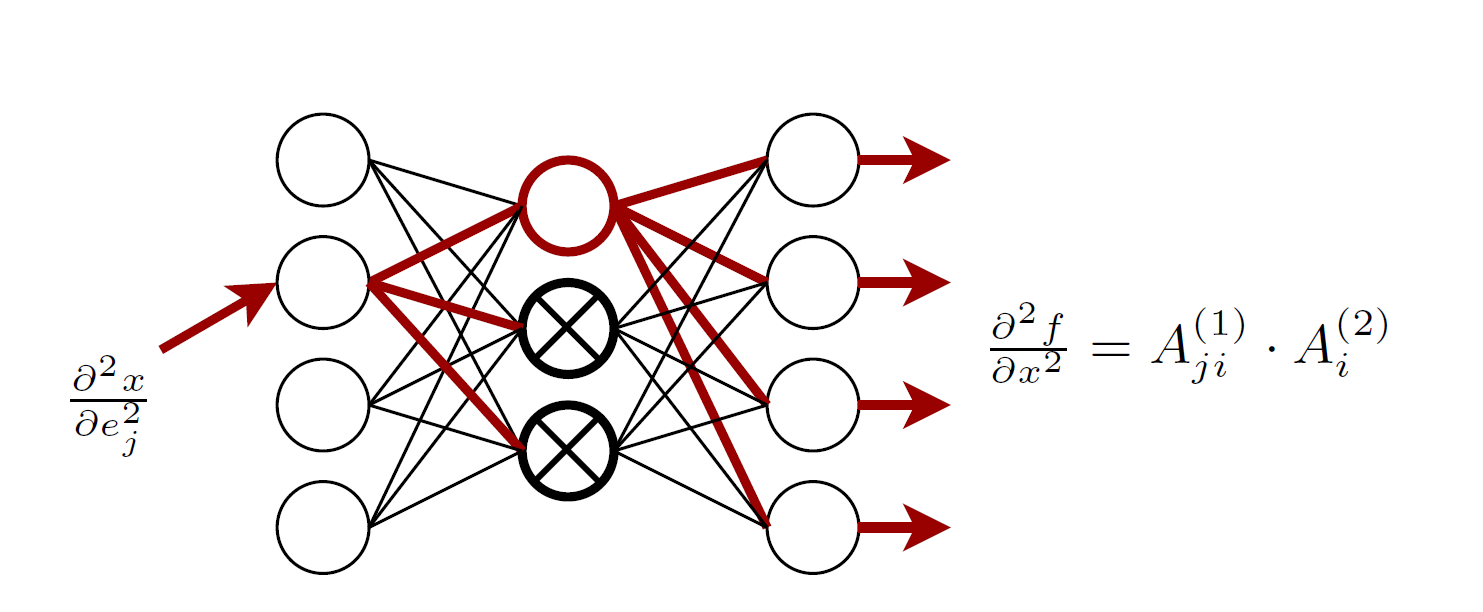
\includegraphics[width=1\linewidth]{1-layer}}
	\caption{Схема атаки на нейронную сеть глубиной 1.}
	\label{ris:1-layer}
\end{figure}

\textbf{Нахождение критических точек.} Для нахождения критических точек анализируется функция, вызываемая DNN, когда входной сигнал $\mathnormal{x}_{1}$ линейно преобразуется в другой входной сигнал $\mathnormal{x}_{2}$. Пусть $\mathnormal{x}_{1}, \mathnormal{x}_{2} \in \mathbb{R}^{d_{0}}$ и  функция $\mu \colon \left[0, 1\right] \to \mathbb{R}^{d_{0}}$, определенная как
$$\mu \colon \lambda \mapsto \mathnormal{x}_{1} + \lambda \left( \mathnormal{x}_{2} - \mathnormal{x}_{1} \right)$$
есть линейное преобразование $\mathnormal{x}_{1}$ в $\mathnormal{x}_{2}$. Это приводит к функции выхода DNN, 
$$\mathnormal{f}^{*}\left( \lambda \right) := \mathnormal{f}\left( \mu \left( \lambda \right) \right),$$
которая является кусочно-линейной функцией с разрывами первого порядка именно тогда, когда один и знейронов переключается между активным/неактивным состояниями.

\begin{figure}[h]
	\centering{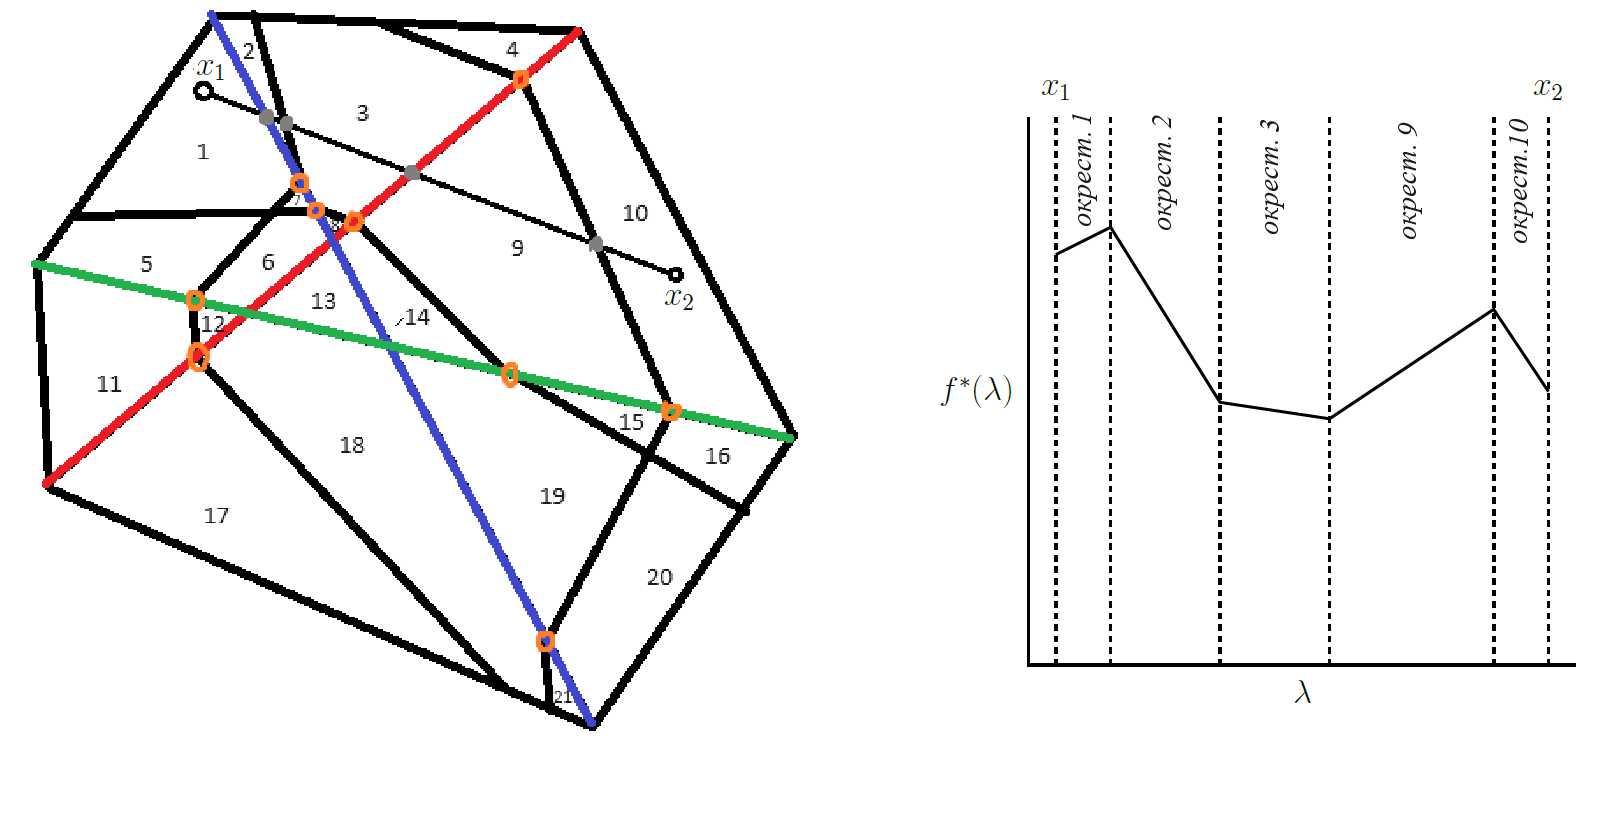
\includegraphics[width=1\linewidth]{lin-razb}}
	\caption{Входное пространство может быть разбито на линейные окрестности,  а выходная функция демонстрирует резкие изменения в поведении при пересечении их границ.}
	\label{ris:lin-razb}
\end{figure}
Как показано на рисунке $\ref{ris:lin-razb}$, мы можем определить разрывы первого пордка и вернуть отображение $\mu$, чтобы восстановить точку, в которой линия от $\mathnormal{x}_{1}$ до $\mathnormal{x}_{2}$ пересекает границу между линейными окрестностями, что является критической точкой для некоторого нейрона.

На практике достаточно измерить наклон графика на рисунке $\ref{ris:lin-razb}$ в разных точках и экстраполировать его, чтобы найти критическую точку, при этом проверяя, нет ли других резких изменений в поведени между ними.

На данном этапе мы ещё не знаем, к какому слою отностится каждая критическая точка, но, выбрав достаточное количество пар $\mathnormal{x}_{1}, \mathnormal{x}_{2}$, в конечном итоге найдутся несколько критических точек для каждого нейрона в сети.

\textbf{Поиск сигнатур.}  Входные данные в DNN $-$ это также вход первого скрытого слоя, и мы имеем полный контроль над ним. Пусть $\eta ~- $ нейрон с весами $\left( a_{1}, \dots, a_{\mathnormal{l}} \right)$. Зная, что $\mathnormal{x}^{*} \in \mathbb{R}^{d_{0}} ~-$ критическая точка для $\eta$, мы можем запросить $\alpha_{i,\;-} = \frac{\partial \mathnormal{f}}{\partial e_{i}}\left(\mathnormal{x}^{*} - \epsilon e_{i}\right)$ и $\alpha_{i,\;+} = \frac{\partial \mathnormal{f}}{\partial e_{i}}\left(\mathnormal{x}^{*} + \epsilon e_{i}\right)$, где $\{e_{i}\}_{i=1}^{d_{0}} ~-$ это канонический базис $\mathbb{R}^{d_{0}}$, а $\epsilon ~-$ маленькое действительное число. Поскольку $\mathnormal{x}^{*}$ является критической точкой, только если либо $\alpha_{i,\;-}$, либо $\alpha_{i,\;+}$ будут иметь $\eta$ в активном состоянии, предполагая, что $\epsilon$ достаточно мал, чтобы никакой другой нейрон не переключился. Разность $\alpha_{i,\;-} - \alpha_{i,\;+}$ содержит градиентную информацию, перемещающуюся от входной координаты $i$ через нейрон $\eta$ к выходу; градиентная информация через все другие нейроны аннулируется. Другими словами, эта разность кратна $a_{i}$, полученной от других слоёв DNN. Деление на другую координату устраняет мультипликативный фактор, т.е. $\left(\alpha_{i,\;-} - \alpha_{i,\;+}\right)/\left(\alpha_{k,\;-} - \alpha_{k,\;+}\right) = {a_{i}}/{a_{k}}$. Если мы зафиксируем $k=1$, восстанавливается сигнатура ($\ref{eq1}$). Обозначим через $\hat {A}_{j}^ {\left(i\right)}$ сигнатуру $j$-ого нейрона слоя $i$, а через $\hat {A} ^ {\left(i\right)} ~-$ матрицу, чьей $j$-ой строкой является $\hat {A}_{j}^ {\left(i\right)}$. Критические точки для одного и того же нейрона в целефом слое 1 будут давать одну и ту же сигнатуру, в то время как критические точки для нейронов в других слоях будут давать разные сигнатуры. Это позволяет нам узнать какие сигнатуры соответствуют нейрону 1-го слоя.

После отслаивания слоя мы также мы также можем определить, соответствует ли сигнатура нейрону в текущем целевом слое, наблюдая за повторениями. Однако, начиная со 2-го слоя, мы уже не можем полностью контролировать вход слоя, и применение вышеописанного метода невозможно (мы не не можем изменять одну координату за раз). Чтобы это преодолеть, в слое $i > 1$, мы выбираем $d_{i} + 1$ направлений $\delta_{k} \sim \mathcal{N} \left(0, \epsilon I_{d_{0}}\right) \in \mathcal{X}$, и пусть $\{y_{k}\} = \{ \partial^{2}\mathnormal{f}\left(\mathnormal{x}^{*}\right) / {\partial \delta_{1} \partial \delta_{k}} \}_{k=1}^{d_{i}}$ и $\mathnormal{h}_{k} = \mathnormal{F}_{i-1}\left(\mathnormal{x}^{*}+\delta_{k}\right)$. Сигнатура тогда получется из вектора $a$ так, что $\left \langle h_{k}, a \right \rangle = \mathnormal{y}_{k}$. Это, однако, даёт частичные сигнатуры (поскольку ReLU на предыдущем слое устанавливает отрицательные значения в ноль). Разные критические точки для одного и того же нейрона дают разные частичные сигнатуры. Каждая частичная сигнатура даёт свой набор координат, и при достаточном количестве частичных сигнатур мы можем восстановить полную сигнатуру.

\textbf{Объединение частичных решений.} Для заданной критической точки $\mathnormal{x}^{*}$ скрытый вектор, полученный из $\mathnormal{f}_{1..i}\left(\mathnormal{x}^{*}\right)$, скорее всего, будет иметь несколько (в среднем, половину) отрицательных нейронов, и, следовательно, $\mathnormal{F}_{i} \left(\mathnormal{x}^{*}\right)$ и любой $\mathnormal{F}_{i} \left(\mathnormal{x}^{*} + \delta_{j}\right)$ будут иметь нейроны, тождественно равные нулю. Это делает невозможным восстановление полного весового вектора с помощью одного применения метода наименьших квадратов $-$ можно вычислить веса только для тех входов, которые не являются нулевыми. Одним из решений может быть поиск критической точки $\mathnormal{x}^{*}$, такой, что по компонентам  $\mathnormal{f}_{1..i}\left(\mathnormal{x}^{*}\right) \ge 0$; однако в общем случае это невозможно.

Вместо этого объединим несколько попыток извлечения весов при помощи процедуры объединения. Если $\mathnormal{x}_{1}$ и $\mathnormal{x}_{2}$ являются критическими точками для одного и того же нейрона, а частичный вектор  $\mathnormal{f}_{1..i}\left(\mathnormal{x}_{1}\right)$ имеет входы $t_{1} \subset \{1, \dots, d_{i}\}$ и частичный вектор $\mathnormal{f}_{1..i}\left(\mathnormal{x}_{2}\right)$ имеет записи $t_{2} \subset \{1, \dots, d_{i}\}$, то можно восстановить соотношения для всех входов $t_{1} \bigcup t_{2}$ путём объединения двух частичных решений, если $t_{1} \bigcap t_{2}$ непустое, как описано ниже.

Пусть $r_{1}$ обозначает извлечённый весовой вектор на критической точке $\mathnormal{x}_{1}$ с входами в локациях $t_{1} \subset \{1, \dots, d_{i}\}$ (соответственно, $r_{1}$ в $\mathnormal{x}_{2}$ с локациями в  $t_{2}$). Поскольку два вектора соответствуют решениям для одной и той же строки матрицы весов ${A}_{j}^ {\left(i\right)}$, вектора $r_{1}$ и $r_{2}$ должны быть согласованы на $t_{1} \bigcap t_{2}$. Поэтому мы будем иметь, что $r_{1} \left |t_{1} \bigcap t_{2} \right| = c \cdot  r_{2} \left | t_{1} \bigcap t_{2} \right|$ для скаляра $c \not = 0$. Пока $t_{1} \bigcap t_{2} \not = \empty$ мы можем вычислить соответствующую константу $c$ и затем восстановить весовой вектор $r_{1,\;2}$ со входами на позициях  $t_{1} \bigcup t_{2}$.

Обратим внимание, что эта процедура также позволяет \textit{проверить}, являются ли $\mathnormal{x}_{1}$ и $\mathnormal{x}_{2}$ критическими точками нейрона $\eta$. Если  $\left | t_{1} \bigcap t_{2} \right | \ge \g$, то до тех пор, пока не существует двух строк $A_{\left(i\right)}$, в которых $\g + 1$ входа скалярно кратны друг другу, будет существовать единственное решение, объединяющее два частных решения вместе. Если процедура объединения проваливается $-$ потому что не существует ни одного скаляра $c$, чтобы  $r_{1} \left |t_{1} \bigcap t_{2} \right| = c \cdot  r_{2} \left | t_{1} \bigcap t_{2} \right| -$ тогда $\mathnormal{x}_{1}$ и $\mathnormal{x}_{2}$ не являются критическими точками одного и того же нейрона.

\textbf{Восстановление знаков с помощью метода замораживания.}  Рассмотрим теперь задачу нахождения знаков текущего слоя. Если сеть не расширяющаяся, эта задача для первого скрытого слоя не представляет сложности. Действительно, для целевого нейрона $k$ в слое $i$, мы можем найти колебание $\mathit{\Delta}_{k}$ во вхоном пространстве, которое производит колебание $\pm e_{k}$ в первом скрытом слое, где $e_{k} \in \mathbb{R}^{d_{i}}$ это базисный вектор в $k$-ом направлении, путём решения $d_{1}$ уравнений в $d_{0}$ переменных, заданных матрицей весов первого слоя. Для любых $\mathnormal{x}$ из входного пространства, выходы нейронной сети в $\mathnormal{x}$ и в ${\mathnormal{x} + \mathit{\Delta}_{k}}$ будут равны, если $k$-ый нейрон не активен в линейной окрестности $\mathnormal{x}$, и будут разными иначе. Эта  простая техника восстановления знаков $-$ "Замораживание".

Есть несколько сценариев, когда этот метод может быть применён к более глубоким слоям. Заметим, что в линейной окрестности любого входа $\mathnormal{x}$, отображение из $d_{0}$-мерного пространства входов в пространство значений, поступающих на слой $i$, является аффинным отображением, поскольку не существует ReLU, переходящих из активного состояния в неактивное или наоборот. Ранг этого отображения определяет, в скольких линейно независимых направлениях мы можем слегка возмущать входы слоя i, когда мы рассматриваем произвольное возмущение входа $\mathnormal{x}$. Если ранг дотаточно высок, мы можем ожидать, что найдём предизображения для каждого базисного вектора и сможем применить метод "Замораживания".

В целом, однако, наши возможности по изменению входов в глубокий скрытый слой сильно ограничены, поскольку около половины нейронов в каждом слое будут подавлены, и, таким образом, ранг аффинного отображения будет уменьшаться по мере продвижения вглубь сети. Метод "Замораживания" может быть применён только в сетях, которые являются "достаточно сократимыми" (то есть размер слоя должен уменьшаться примерно в 2 раза в каждом слое, чтобы компенсировать потерю ранга).